\hfill\break

This chapter addresses the mechanisms through which AKF generates and
documents its outputs, as seen in \autoref{fig:output-simple}. More
specifically, this covers the modules and submodules seen in
\autoref{fig:output-full}. The submodules for the \emph{virtual machine}
and \emph{action automation library} have been omitted for brevity.
(Note that the ``imaging library'' and ``validation library'' are
theoretical submodules that would fulfill the ``after the fact''
analysis described in \autoref{human-readable-reporting} and are not currently implemented.)

\begin{figure}[htbp]
\centering
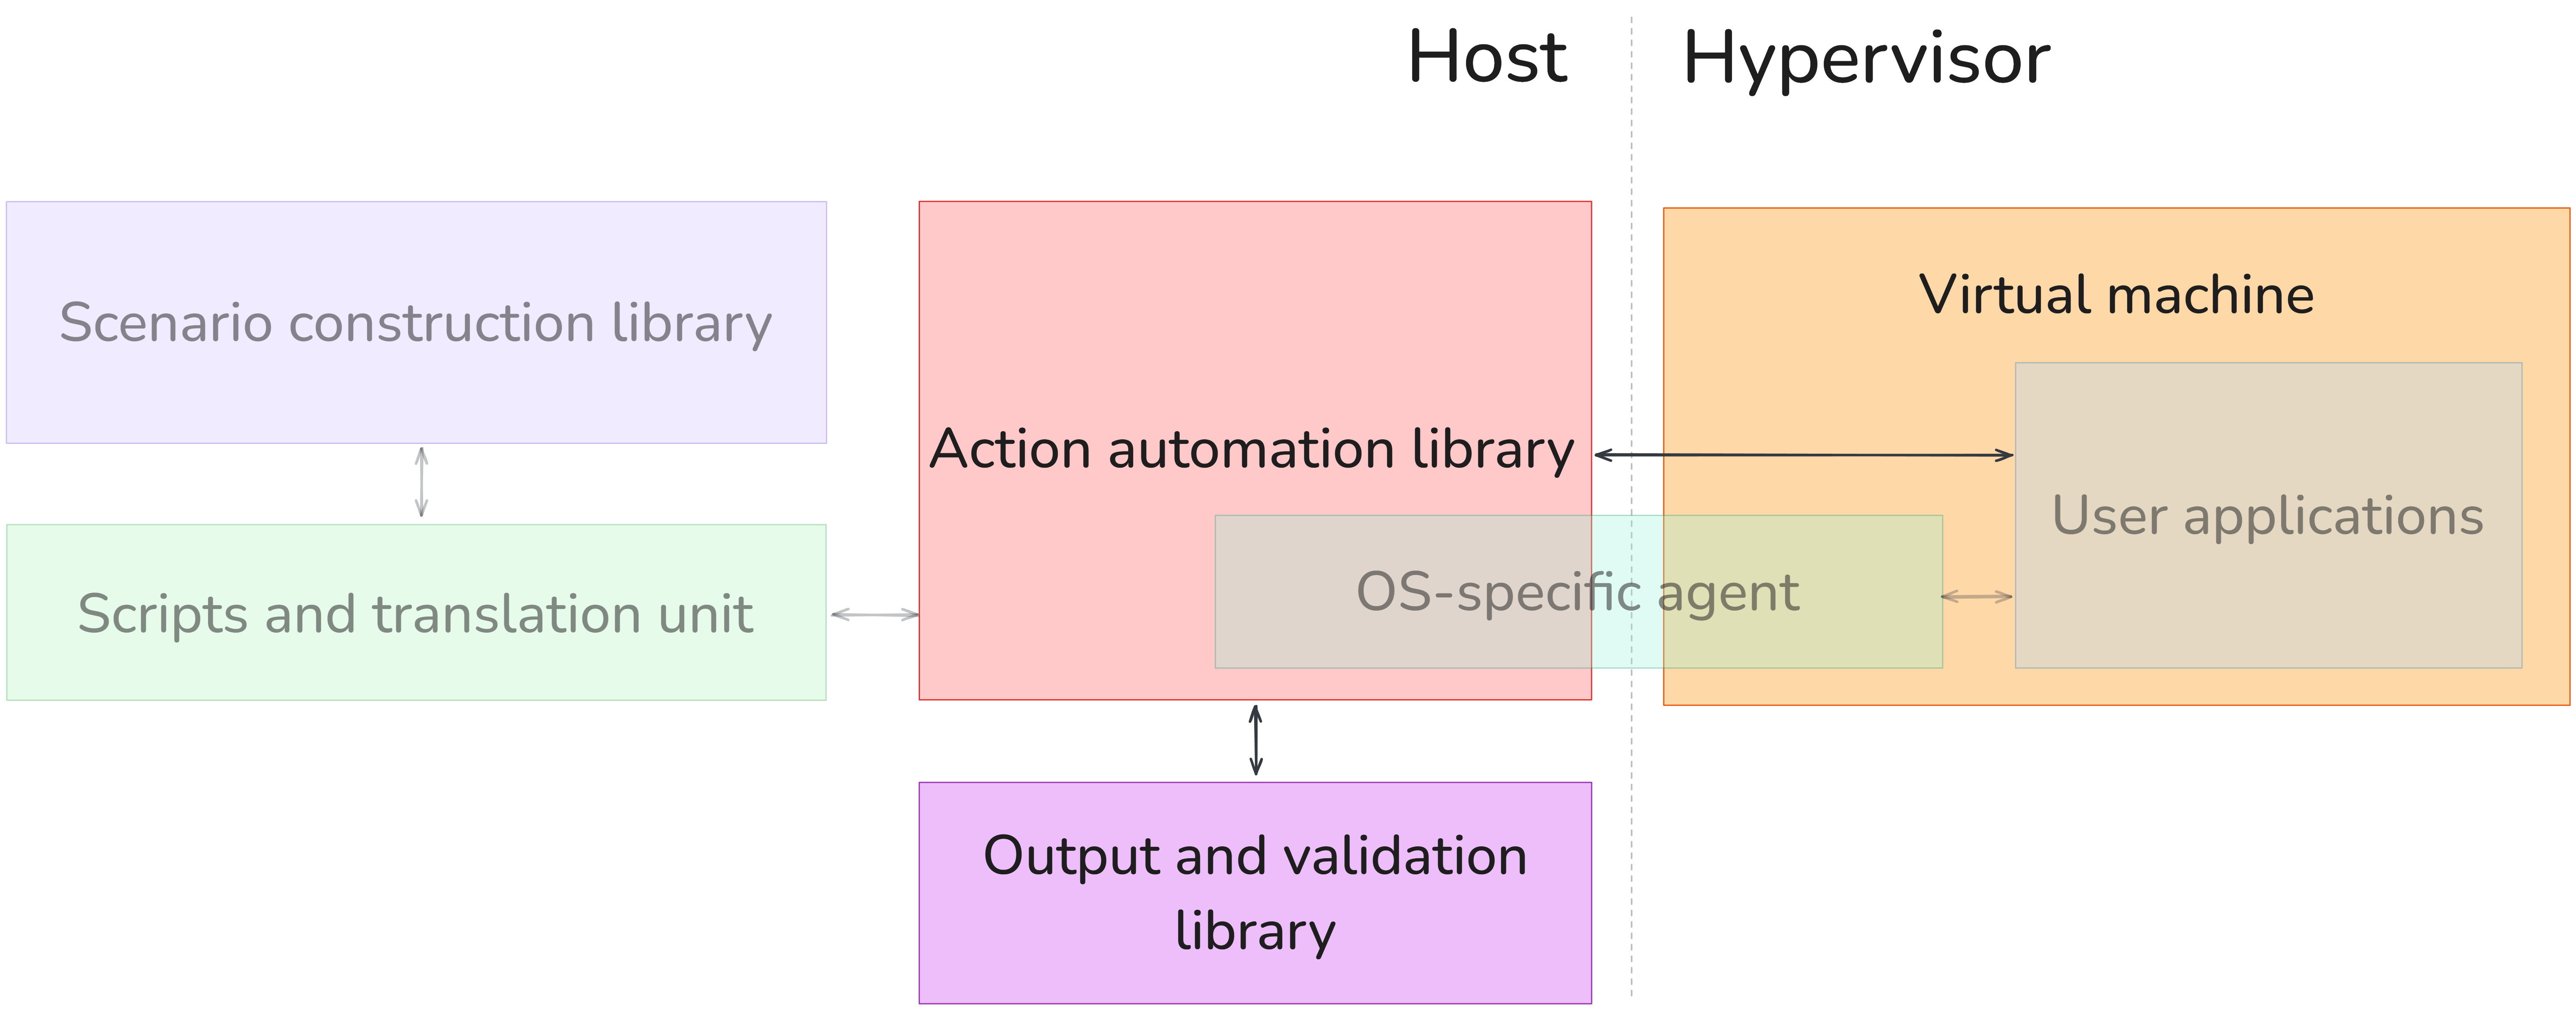
\includegraphics[width=1\linewidth]{output-and-validation-simple.png}
\caption{Simplified AKF architecture diagram for output and validation
modules}\label{fig:output-simple}
\end{figure}

\begin{figure}[htbp]
\centering
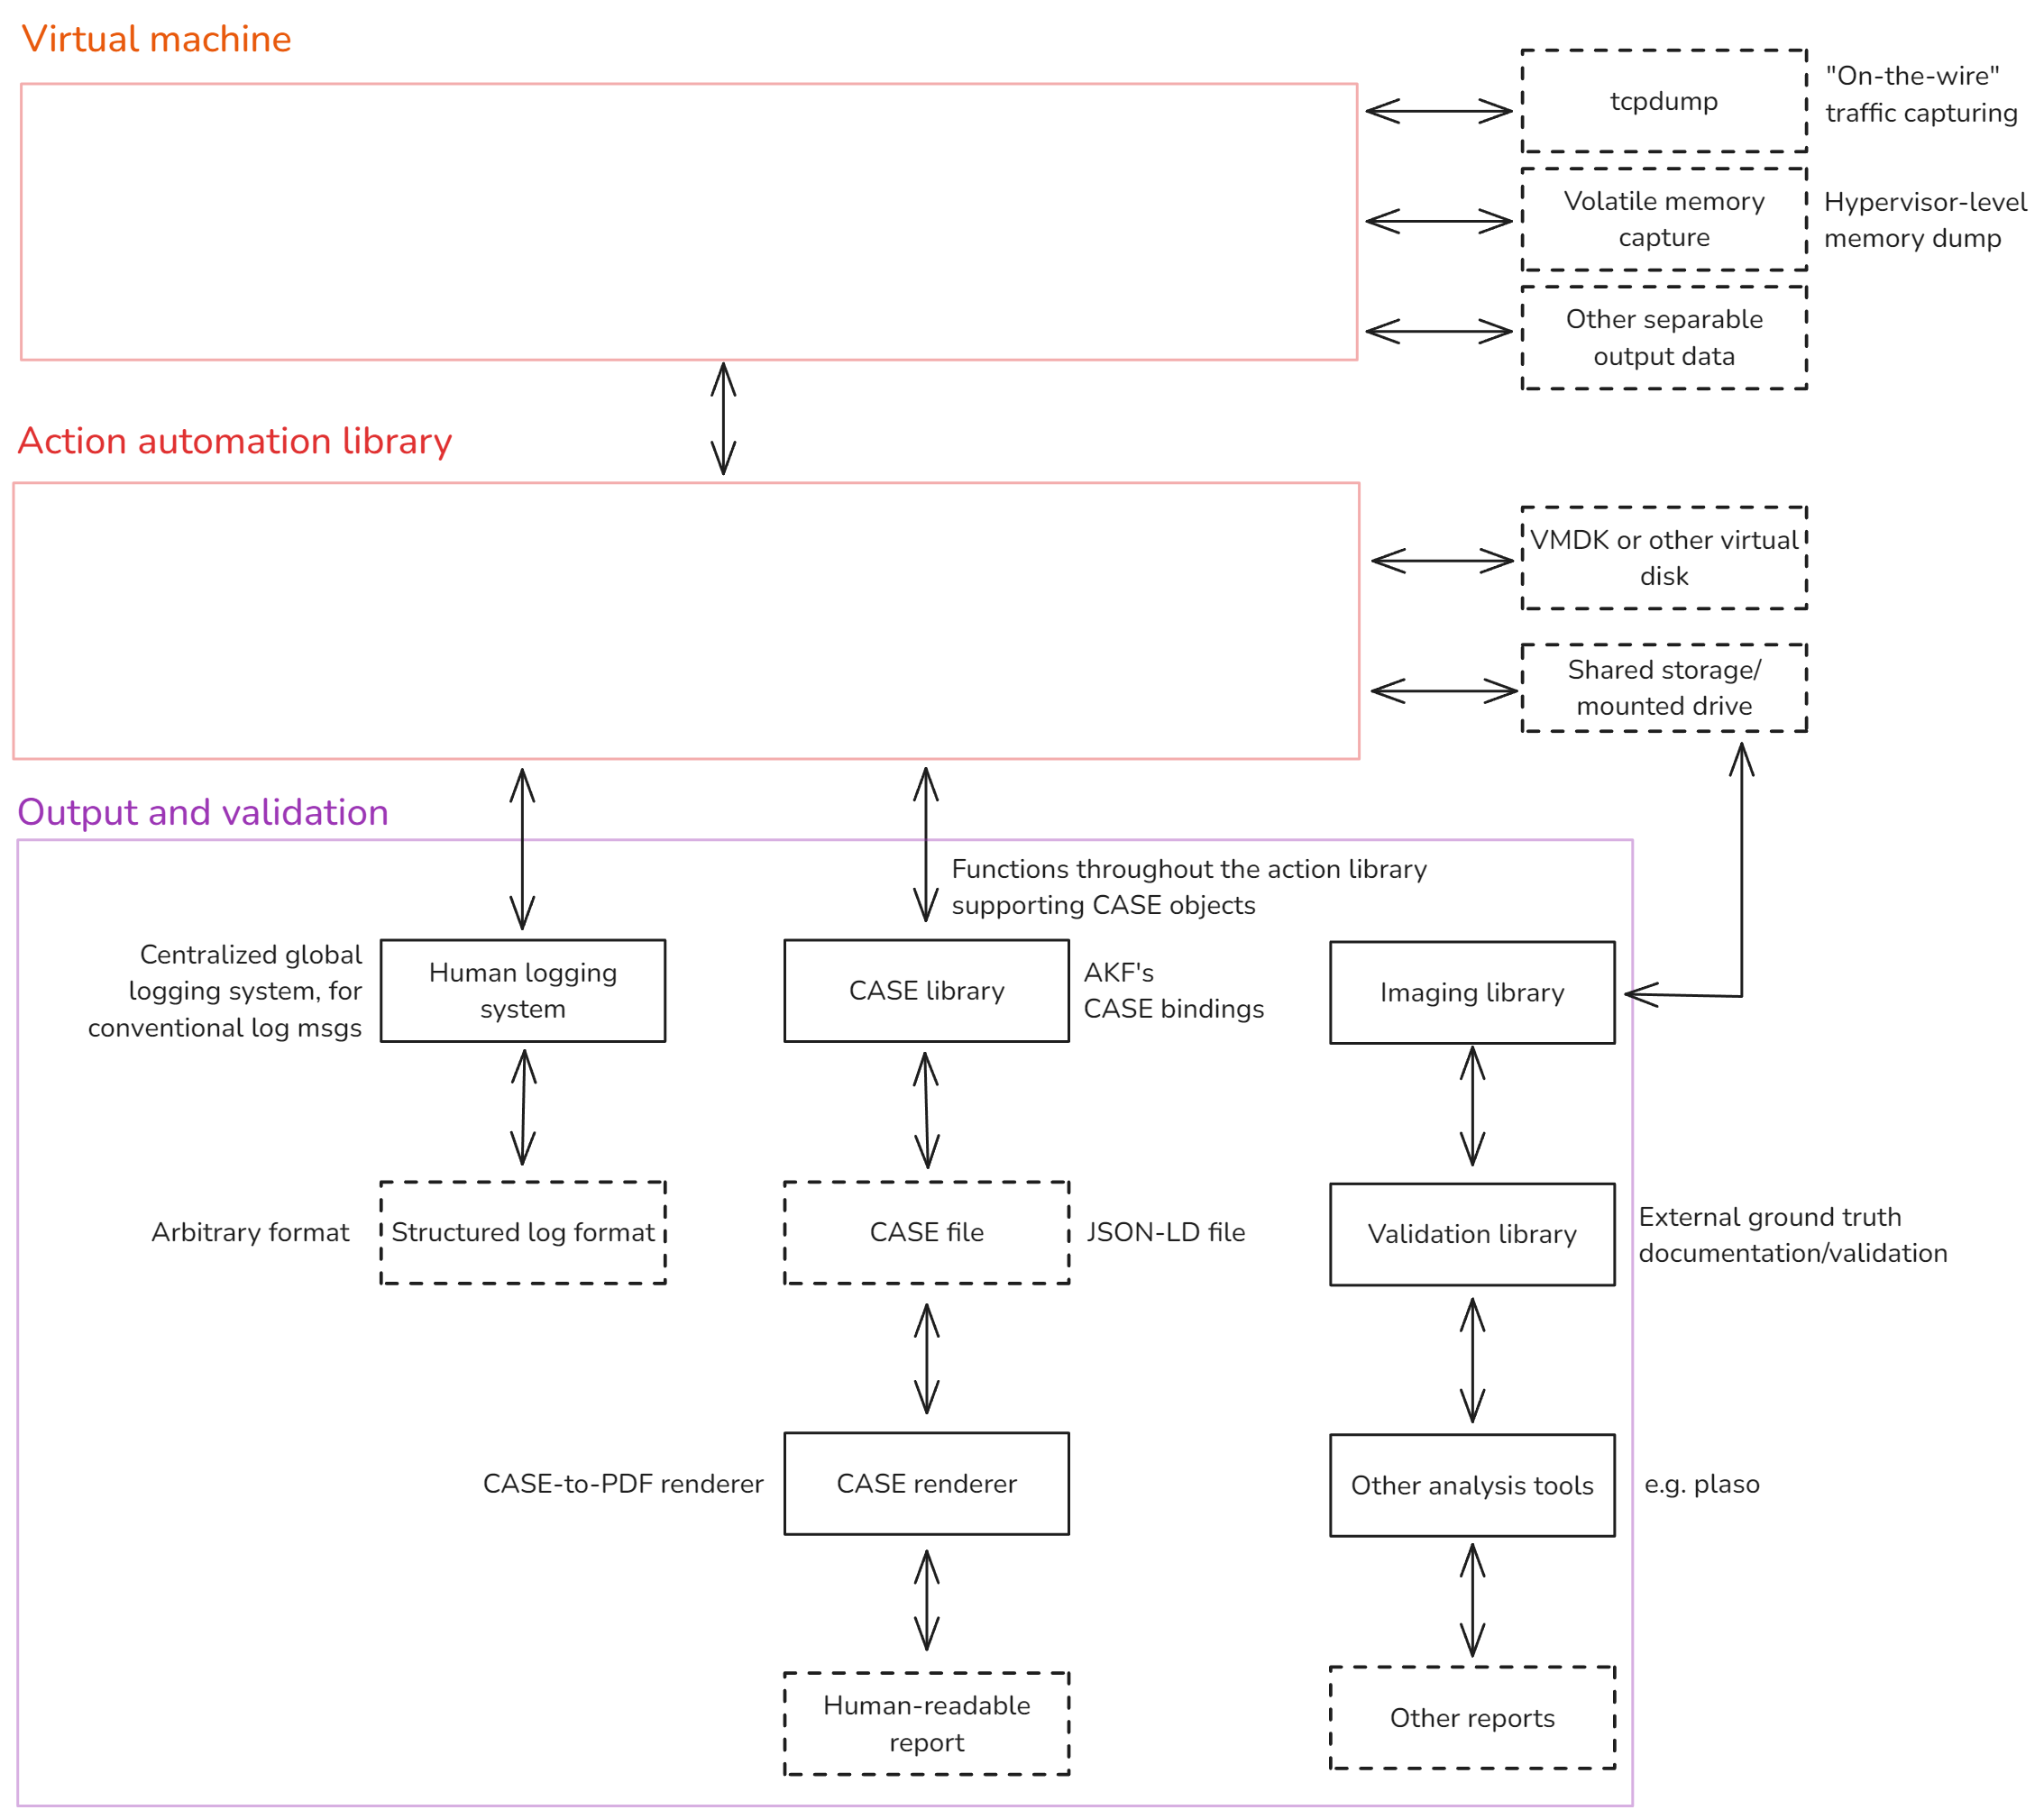
\includegraphics[width=1\linewidth]{output-and-validation-full.png}
\caption{Abridged diagram of AKF modules related to output and
validation}\label{fig:output-full}
\end{figure}

Whether generating artifacts through physical or logical means, these
artifacts must ultimately be exported and documented. In most cases,
this involves generating disk images, volatile memory captures, or
network captures; additionally, individual artifacts, such as browser
history, may be selectively extracted from a filesystem. Disk, memory,
and network captures will be referred to as ``core outputs'' throughout
this chapter to distinguish them from ``standalone'' artifacts. Both can
be broadly described as ``outputs'' of a scenario.

The contents and details of these artifacts, as well as the means
through which they were generated, should be documented in a structured
format. This ground truth should fully describe the contents of a
forensic dataset; that is, it should identify every artifact that can be
discovered within a dataset and every action taken to plant those
artifacts. This metadata, in addition to core outputs and standalone
artifacts, comprises a forensic dataset.

From an educational perspective, the ground truth represents an ``answer
key'' to the dataset; it details every artifact of interest that an
analyst could be expected to discover. For research, it allows for
well-labeled datasets that can be used for tool development, validation,
and testing. Ideally, this should be generated independently of the
input script used to construct the scenario. This allows \emph{all}
artifacts to be documented, including those not explicitly declared or
deemed significant by the scenario creator.

This chapter addresses the role of the output and validation library in
providing several AKF services, including a centralized logging system,
CASE object generation, and the generation of outputs such as disk
images, network captures, and volatile memory dumps. In particular, it
describes the reporting and documentation functionality enabled by CASE
and the role that this metadata plays in ensuring dataset
reproducibility and supporting community usage.

\section{Core outputs}\label{core-outputs}

In the same way that artifacts can be generated through logical and
physical means, outputs can also be generated through logical and
physical means. Some of these are analogous to techniques used by
real-world investigators to extract forensically sound evidence that is
valid in a court of law; others are less suitable in formal settings but
still have valid use cases.

Logical output generation refers to any technique in which software is
used inside a running virtual machine to generate these outputs. This
includes using software such as FTK Imager
\cite{exterroFTKImagerForensic} to capture the volatile memory of a
device or construct a \emph{logical} disk image. Similarly, network
captures can be created by simply running Wireshark on the target
device. Individual artifacts can be copied off the device by hand and
sent to a network or removable drive.

Physical output generation refers to techniques in which the operating
system is unaware of the technique, leaving few or no traces in the
resulting outputs. In practice, this involves using tools such as
hardware write blockers to extract disk images and network taps (or
another traffic mirroring solution) to capture traffic over a particular
interface. Although challenging, a physical extraction of RAM is also
possible by performing a ``cold boot attack.'' RAM sticks can be cooled
to low temperatures before being removed from a running machine, slowing
the process of memory decay as a result of the DRAM cells being
unpowered \cite{yitbarekColdBootAttacks2017}.

AKF directly supports physical output generation for all three core
outputs and indirectly supports logical output generation for core
outputs and standalone artifacts. Physical output generation for virtual
machines is generally achieved through direct interaction with the
hypervisor.

\begin{itemize}
\tightlist
\item
  For \textbf{disk images}, the output can simply be the virtual hard
  drive used by the hypervisor on the host machine (such as VDI files
  for VirtualBox). If a standard raw disk image is desired, the
  command-line tool VBoxManage supports converting various virtual drive
  formats to raw disk images using the
  \passthrough{\lstinline!vboxmanage clonemedium!} command. This expands
  the compacted virtual drive to the ``declared'' size of the drive as
  seen by the operating system, allowing it to be bootable on actual
  hardware.
\item
  For \textbf{network captures}, VirtualBox allows the user to enable
  network tracing over multiple interfaces, dumping network traffic as a
  .pcap file on the host machine. This can be enabled or disabled at any
  time without affecting network connectivity or the state of the
  virtual machine.
\item
  For \textbf{volatile memory dumps}, VBoxManage provides the command
  \passthrough{\lstinline!vboxmanage debugvm <machine\_name> dumpvmcore!},
  which creates an ELF core file of the virtual machine's volatile
  memory that can be analyzed using a tool such as Volatility
  \cite{volatilityfoundationVolatility32025}.
\end{itemize}

These physical output options are often sufficient to generate datasets.
If only specific files are desired, the existing file transfer utilities
provided by AKF can be used to extract standalone artifacts. Users can
also manually perform the logical techniques described above (such as
running Wireshark or installing FTK Imager) through various means. For
example, a user can pause an AKF script until instructed to continue;
during this time, the user can manually run FTK Imager to extract the
contents of RAM.

The logic for generating physical outputs is contained in the opaque
submodules seen in \autoref{fig:output-a}.

\begin{figure}[htbp]
\centering
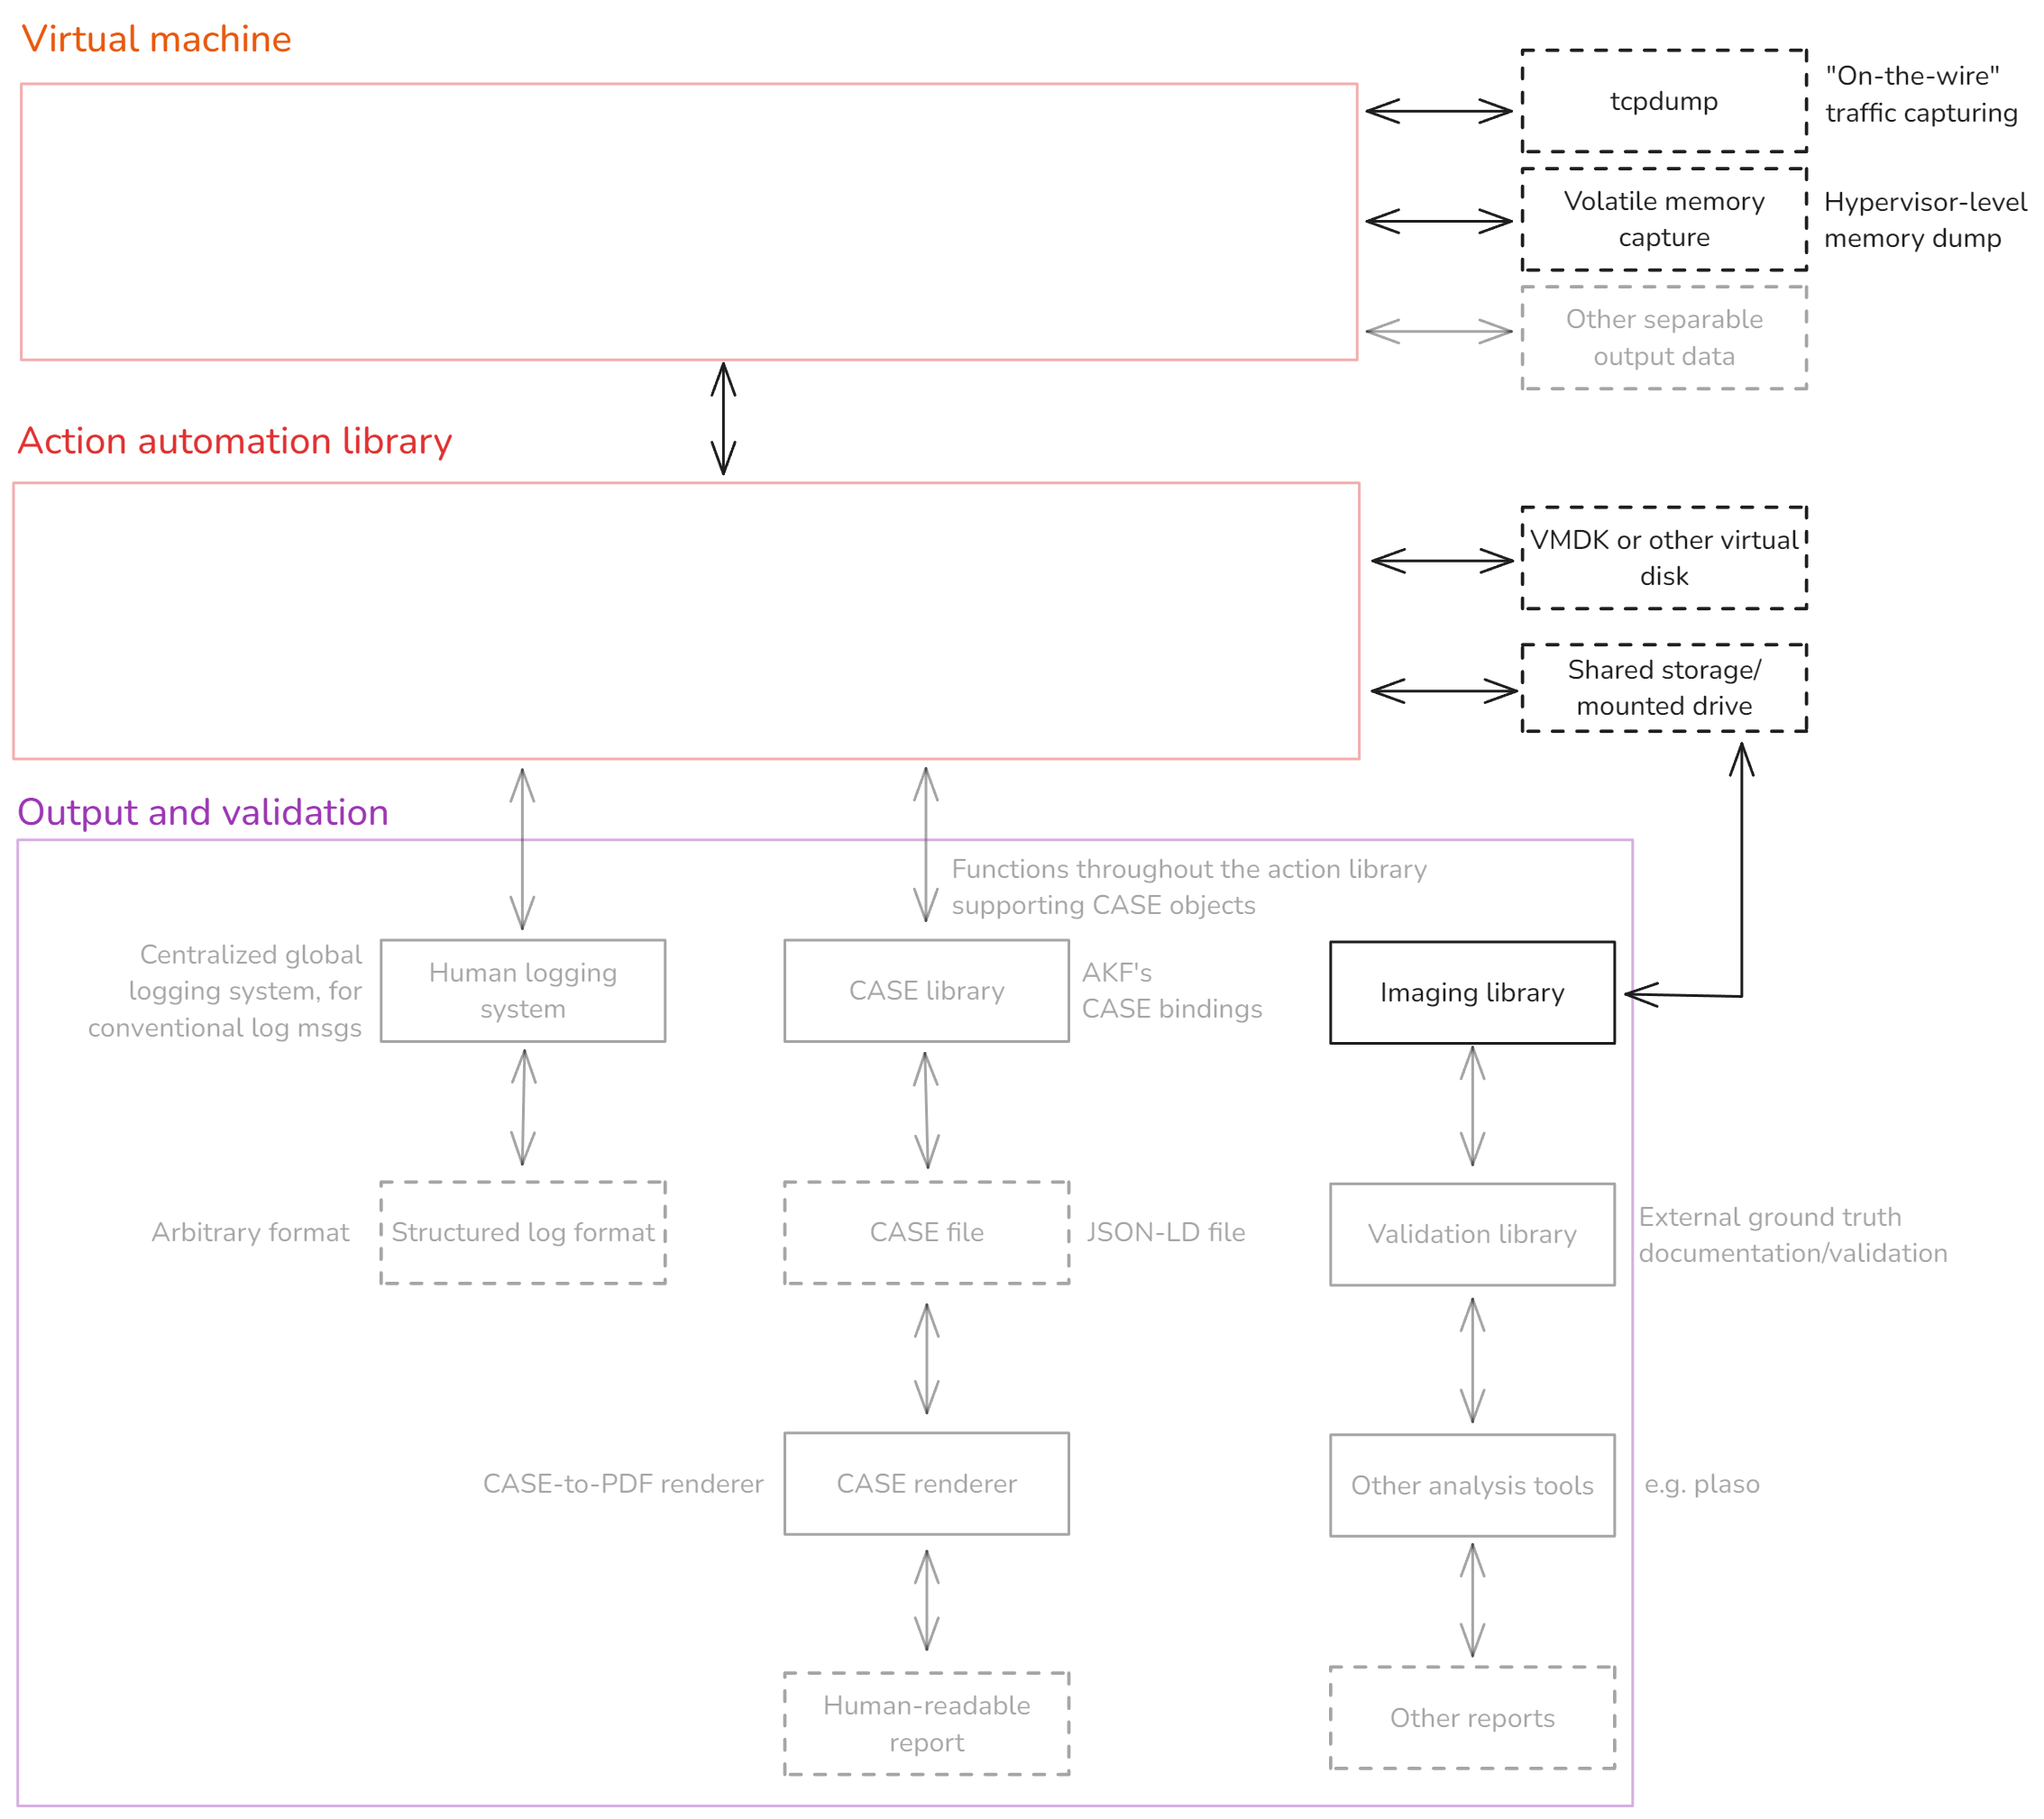
\includegraphics[width=1\linewidth]{output-and-validation-a.png}
\caption{Diagram of AKF modules related to physical output
generation}\label{fig:output-a}
\end{figure}

\section{Metadata and ground
truth}\label{metadata-and-ground-truth}

There exists a gap in the ability of instructors and researchers to
perform bulk searches for specific forensic artifacts in public
datasets. For example, the NIST CFReDS repository
\cite{nationalinstituteofstandardsandtechnologyCFReDSPortal}, one of
the largest listings of forensic datasets, does not have a unified
standard for describing uploaded images. Although users can search by
keywords and human-applied tags, metadata is not available in a
standardized format.

For many datasets, an instructor or researcher must read through a PDF
answer key (if one exists) or analyze the image themselves to determine
if a particular artifact is present. Answer keys are not inherently
machine-readable and are not suited for identifying specific artifact
types in bulk. Additionally, the content of human-made reports may be
limited to what the author believes is significant, even if other
artifacts of interest are present in the image. In turn, it may be
difficult to quickly determine if a dataset is useful in demonstrating a
particular technique to students or validating a specific feature of a
newly developed tool.

A rigid, well-defined format for ground truth is invaluable to
researchers engaging in tool validation and development. Perhaps the
lack of labeled forensic datasets on major repositories can be
attributed to the lack of a need for one; Grajeda et al.~demonstrated
that scenarios are rarely shared between researchers, so there is seldom
a need to label them for general-purpose usage. AKF has the opportunity
to solve this issue through the mass production of labeled datasets
adopting a single established standard.

Many forensic analysis tools support exporting investigation details in
both proprietary and language-agnostic formats, though these are not
always suitable for generating ground truth. For example, Cellebrite's
UFED supports exporting to UFDR and XML files, Magnet Axiom supports
exporting to XML, and Autopsy supports a variety of formats, including
Excel, STIX, and HTML. Each format varies in structure and content and
does not necessarily contain equivalent information for the same
analyzed disk image using default settings. This is the primary
challenge with using an existing format, particularly a proprietary
format subject to vendor changes; details for certain artifact types may
be missing or change without warning. Many prior synthesizers (including
AKF) also generate human-readable log messages during artifact
generation, though this is rarely suitable for documenting the contents
of a dataset.

There has been extensive work in other fields towards developing a
structured ontology that describes relationships and low-level details.
This includes the EVIDENCE project for criminal justice and the
Structured Threat Information Expression (STIX) format for conveying
cyber threat intelligence
\cite{caseyLeveragingCybOXStandardize2015}. For example, STIX
provides a standard set of objects that allows organizations to describe
observed attacker techniques and associate them with specific pieces of
malware, attack campaigns, or threat actors.

However, there have been few efforts to document the contents of a
forensic scenario (disk images and related metadata) in a vendor-neutral
manner. One such format was developed by Abbott et al., who provide an
XML-based notation of events in a dataset
\cite{abbottAutomatedRecognitionEvent2006}. However, the
specification does not appear to be available or maintained as part of
another project. Similarly, although not designed to document technical
details in a dataset, Conlan et al.~describe a taxonomy for describing
anti-forensic techniques at a high level that could be integrated into a
scenario description language
\cite{conlanAntiforensicsFurtheringDigital2016}. Neither of these
formats appear to be supported by community tools, nor do they fill the
need for low-level, queryable dataset descriptions.

Besides limited community support for and adoption of existing formats,
Casey et al.~found that these formats lacked features such as
parent-child relationships, user actions, and non-technical case
information such as a chain of custody. In response, the same authors
introduced the Digital Forensic Analysis eXpression, or DFAX, a language
extending CybOX (the predecessor to STIX) for use in the digital
forensics community. DFAX later became the Cyber-investigation Analysis
Standard Expression (CASE)
\cite{caseyAdvancingCoordinatedCyberinvestigations2017}. CASE is
perhaps the most comprehensive and actively supported ontology available
for digital forensics, with support from both NIST and the Linux
Foundation. As a result, AKF uses CASE as its primary format for
documenting datasets, deliberately including support for CASE throughout
various libraries.

\subsection{CASE and Python
bindings}\label{case-and-python-bindings}

CASE is a vendor-neutral format designed to document both technical and
non-technical information about a digital forensics case
\cite{caseyAdvancingCoordinatedCyberinvestigations2017}. It aims to
cover as many OS-specific and application-specific artifacts as possible
while still providing the flexibility to describe artifacts from
uncommon applications. In theory, data exported from any major vendor,
such as Cellebrite, Magnet, or FTK, can be converted into a valid CASE
file. CASE is an extension of the Unified Cyber Ontology, or UCO, which
provides basic objects not specific to digital forensics (such as
applications or users). Consistent with the CASE project's
documentation, references to CASE and CASE/UCO throughout this chapter
refer to the same project.

CASE is built on the Resource Description Framework (RDF), a model for
describing information using relationships. Two objects are linked using
a predicate, with the set of three elements forming a ``triple.'' This
pattern allows for directed, labeled graphs to be expressed using RDF.
The ontology of CASE objects is defined using the Terse RDF Triple
Language, or Turtle, which allows these triples to be written in a
simple text format. In many ways, the Turtle definitions can be seen as
the class definitions for CASE objects; instances of these objects can
be expressed in JSON-LD, an extension of JSON for linked data. A
collection of CASE objects is known as a bundle; applications can add
instantiated CASE objects to a bundle as needed.

Because the CASE format itself is language-agnostic, it is necessary to
write language-specific libraries that allow for instantiating CASE
objects. At the time of writing, the CASE project provides Python
bindings for UCO/CASE version 1.4 \cite{CaseworkCASEMappingPython}.
Each unique object type is represented as a Python class, which can be
instantiated to produce individual objects. However, this library has
several limitations due to its design; for example, CASE objects are
internally represented as a dictionary of strings rather than a set of
instance variables. While this makes it easier to serialize CASE objects
to JSON-LD dictionaries, modifying objects after they have been
instantiated is extremely difficult.

It is also worth noting that each object in the CASE ontology appears to
have been manually translated to its corresponding Python class
definition. This is slow and time-consuming, especially given that a
significant overhaul of UCO/CASE to version 2.0 is underway with new
object definitions \cite{UcoProjectUCODevelop2002025}; there appears
to be no active effort to update the 1.4 bindings to 2.0.

AKF leverages and contributes Pydantic-based bindings for CASE. The
foundation for this system is the Pydantic library for Python, which
allows developers to quickly define classes (referred to as ``Pydantic
models'' or simply ``models'') with built-in schema validation and
serialization based on Python type hints \cite{colvinPydantic2024}.
More broadly, Pydantic allows us to simplify the declaration of
individual objects while providing runtime type validation and automatic
casting.

Examples of CASE-related definitions and a detailed comparison of AKF's
bindings compared to the existing CASE bindings can be found in
\autoref{case-python-bindings}. One notable example
from this section is the simplification of a CASE object declaration
from 35 lines in the existing CASE bindings to only eight lines in AKF.
These simple declarations are possible primarily because the conversion
of objects to valid JSON-LD elements is deferred until serialization
instead of converting objects to dictionaries immediately upon
instantiation. This design choice allows us to centralize the
serialization logic in a single parent class that all CASE objects
inherit from. In exchange for slightly increasing the complexity of
converting objects to a dictionary with the correct key names, we can
massively simplify the logic for declaring individual CASE objects.

A script is provided with AKF's CASE bindings to automatically parse the
RDF files and convert them to valid Pydantic models. It automatically
converts XSD datatypes to their native Python types (or a custom wrapper
type if a native type does not exist), correctly inherits classes, and
automatically generates docstrings and Pydantic fields as applicable.
The script also topologically sorts dependencies in the same file; an
RDF object's ``parent'' class may be declared \emph{after} its ``child''
class, which is disallowed in Python. This dramatically simplifies the
process of maintaining Python bindings for UCO/CASE, as well as the
overall design of the library for future needs.

Note that there are certain inconsistencies between the Turtle CASE
definitions and those of AKF. These issues are also true of the public
bindings for CASE/UCO 1.4 that are currently available; this is not
unique to AKF's Pydantic-based implementation. These are described in
greater detail at the end of \autoref{case-python-bindings}.

\subsection{CASE integration in
AKF}\label{case-integration-in-akf}

AKF's CASE Python bindings are integrated throughout artifact-generating
libraries in AKF. This is depicted through the opaque submodules in
\autoref{fig:output-b}.

\begin{figure}[htbp]
\centering
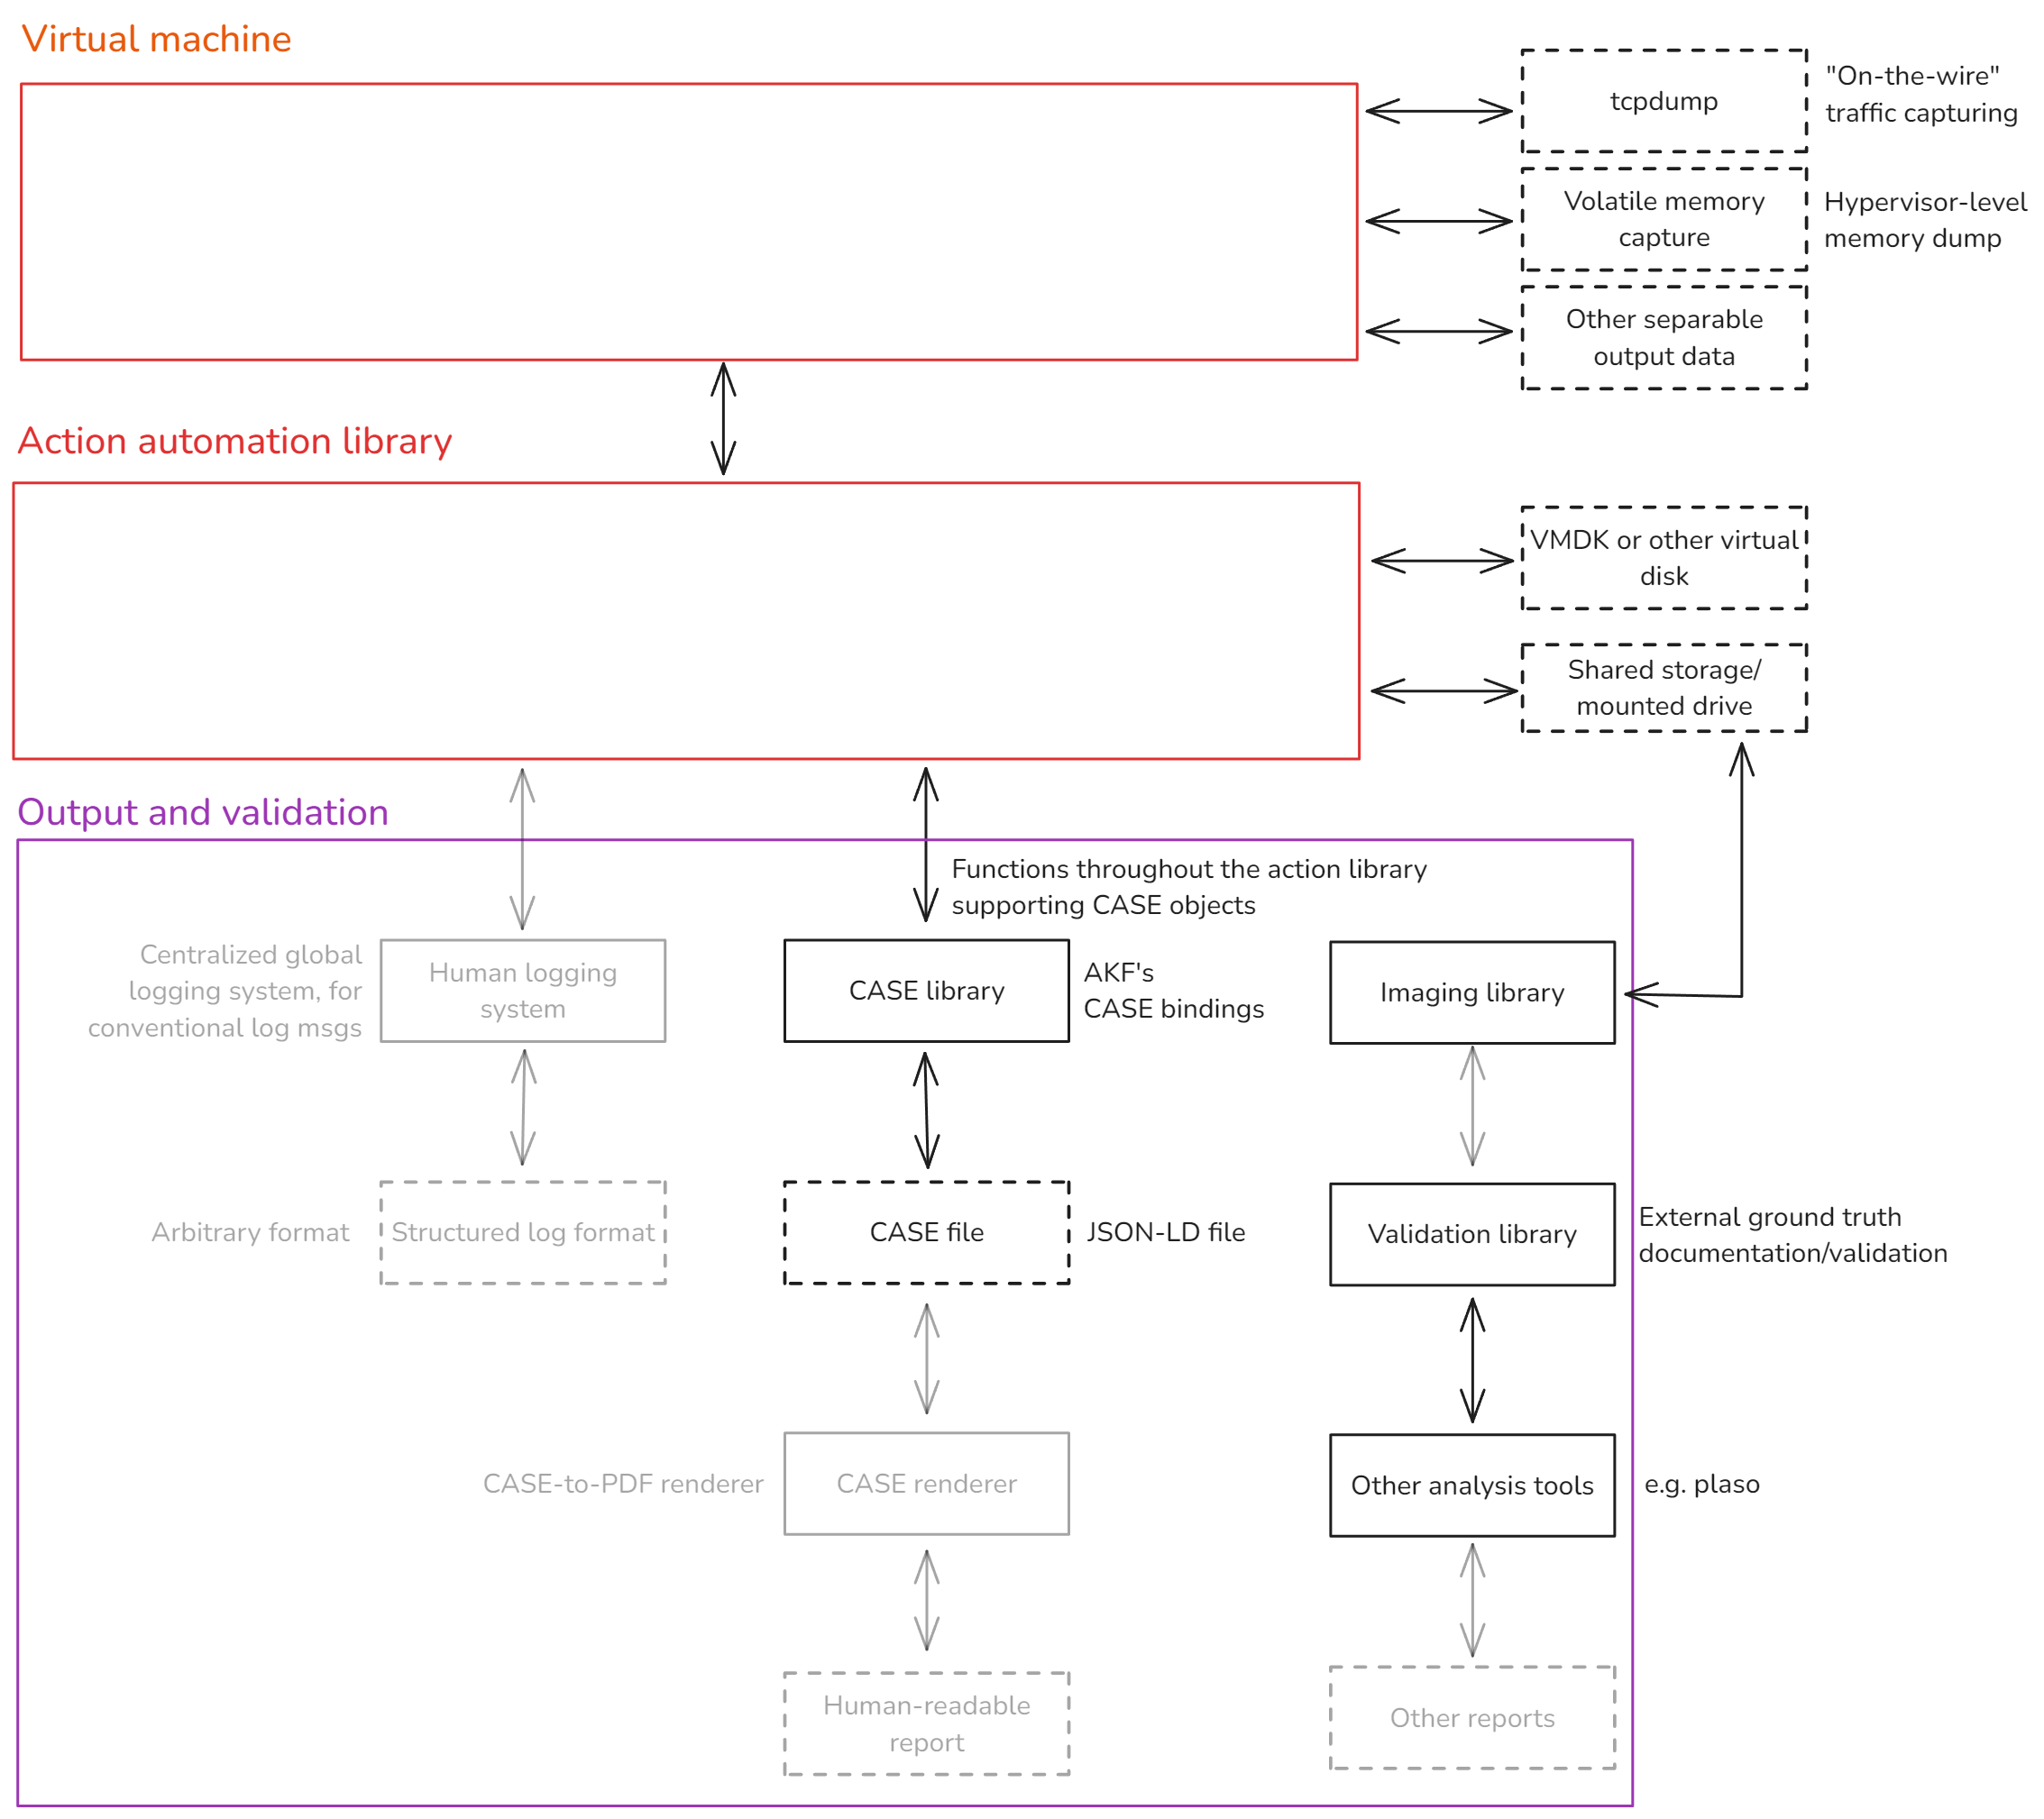
\includegraphics[width=1\linewidth]{output-and-validation-b.png}
\caption{Diagram of AKF modules related to CASE object
generation}\label{fig:output-b}
\end{figure}

There are two distinct points at which CASE artifacts can be generated
and attached to a scenario -- during scenario generation and after
scenario generation.

Various functions and classes throughout the AKF core libraries and
agent API accept an optional CASE bundle when invoked or instantiated.
As CASE-compatible functions are called, they can automatically add CASE
objects corresponding to the artifacts generated through their
execution. For example, if the agent subservice API for automating
Chromium browser actions is provided with a CASE bundle, navigating to a
page using the API could automatically generate a CASE object describing
the page visit and add it to the bundle. This process can occur entirely
within the host, allowing CASE-related logic to remain out of the agent
where needed.

However, recall from \autoref{the-akf-agent} that using RPyC for agent communication allows AKF to pass
complex objects between the agent and the host machine. This includes
CASE bundles and objects, as well. For example, suppose that a CASE
object must be made for a file downloaded from the internet that
frequently changes location, size, and content. The resulting CASE
object can only be accurately constructed using some form of agent-side
analysis as the action occurs. Once instantiated, the object can be
returned to the host machine to append to a larger CASE bundle.

Some CASE ontology objects, such as those describing Windows prefetch
files, are best constructed when disk images and other core outputs are
created. For example, it is possible to create CASE prefetch objects
during the execution of a scenario. However, these objects are likely to
become outdated if their corresponding applications are launched later
in the scenario, thus changing the content of the prefetch files and
making the existing CASE objects inaccurate.

In turn, to make the generation of such objects more efficient and
accurate, certain CASE objects must be instantiated ``after the fact'';
that is, they cannot or should not be automatically generated as part of
AKF automation routines. This can be trivially achieved by analyzing
core outputs (such as disk images) using independent tooling. Such tools
might include general-purpose DFIR tools that support CASE objects (such
as Autopsy) or tools that explicitly focus on constructing CASE objects
(such as tools built with the official or AKF Python bindings for CASE).

However, ``after the fact'' analysis can also be achieved on live
virtual machines using existing AKF design patterns. In particular,
agents may have RPyC subservices whose sole purpose is to generate CASE
objects. For example, the \passthrough{\lstinline!artifacts!} subservice
mentioned in \autoref{the-akf-agent}
can collect Windows prefetch files immediately before a disk image is
created, allowing it to construct CASE prefetch objects that reflect the
disk image without requiring separate tooling. CASE-oriented
functionality can also be implemented in existing subservices; for
example, the \passthrough{\lstinline!chromium!} subservice can create
CASE objects for Chrome and Edge browser history after all browser
automation actions have been performed. This allows the dataset to be
documented independently of synthesizer actions intended to emulate
human activity -- a desirable feature identified at the beginning of
this chapter.

The flexibility of these two approaches -- enabled by CASE's deep
integration into AKF -- makes it possible to construct CASE objects in a
manner that requires little additional effort by scenario developers.
Scenario developers do not need to be concerned with instantiating their
own CASE objects when using high-level APIs so long as an AKF library
developer has written support for automatic CASE object construction.
This significantly reduces the need for scenario developers to construct
ground truth information by manually analyzing synthesizer-created
outputs.

By extension, this means that the detailed documentation of AKF outputs
is innate to many scenarios constructed using AKF. Lowering the effort
required to document an AKF-generated scenario improves the likelihood
that any public AKF scenario can be immediately valuable (or determined
to be valuable) to researchers and educators. This significantly
contributes to AKF's goal of supporting an ecosystem around its images;
the CASE bundles of many scenarios can be queried in bulk to identify
datasets that might be useful for a specific purpose without having to
download the dataset itself. This information can also be used to
identify and analyze broader trends across scenarios, such as the
frequency of a particular artifact appearing in all Windows datasets.

While this machine-readable reporting significantly improves the ability
of the forensic community to locate useful datasets, it is verbose and
unsuitable as a human-readable summary. Human-readable reporting is
particularly relevant in a classroom setting, where the distribution of
simplified answer keys to graders and students focusing on key artifacts
is preferable to the exhaustive reporting provided by a CASE bundle.
This leads us to the following section, which briefly addresses the
conversion of AKF-generated metadata into human-readable reports.

\section{Human readable reporting}\label{human-readable-reporting}

As alluded to in the previous section, converting a rigid, well-defined
format to a human-readable format is often easier than performing the
reverse operation. Indeed, this is the approach taken by AKF, which does
not create human-readable reports as an immediate output of dataset
generation. (AKF generates human-readable log files during artifact
generation, but these are unstructured and are created primarily for
debugging rather than analysis.) Instead, AKF supports a simple yet
flexible system for generating human-readable PDF reports from existing
CASE bundles after generating a dataset.

AKF implements human-readable reporting through a set of ``renderers,''
which focus on analyzing specific artifacts found in a CASE bundle and
generating human-readable content. Each renderer accepts a complete CASE
bundle and extracts CASE objects of supported types; the renderer then
uses the information contained in these objects to generate a Markdown
document, which can include formatted text, tables, images, and other
elements that may be useful to a human. The results of each renderer are
combined to form a larger Markdown document (or documents) with multiple
sections, one for each renderer. The combined document can be converted
to a PDF using Pandoc \cite{macfarlanePandoc2025}, a general-purpose
tool for converting between documents of various types. Users can modify
the generated Markdown documents before running Pandoc, if desired.

A single CASE bundle can be passed through as many or as few renderers
as needed to generate a suitable report for a dataset. So long as the
original CASE bundle is available, users can reanalyze datasets with
arbitrary renderers; this means that dataset reports can be regenerated
with as much detail as a user needs for a specific use case.
Furthermore, if new renderers are developed for artifacts that are
present in older datasets, the human-readable report can be regenerated
to include these artifacts.

This modular, ``evergreen'' approach to reporting allows these reports
to be interpreted as a focused snapshot of what a dataset contains.
Importantly, this can be done without compromising the dataset itself;
the CASE bundle remains the single, comprehensive source of truth.
Contrast this with human-written PDF reports, which may contain human
biases and are rarely maintained in older datasets.

\autoref{fig:scenario-report} shows a page taken from a sample report.
The information contained in this report was derived from collected
\passthrough{\lstinline!WindowsPrefetch!} and
\passthrough{\lstinline!URLHistory!} CASE objects, which were then
passed through their associated renderers. Each renderer generated
Markdown documents containing the information in the report, which were
then combined and converted to a PDF with Pandoc. (Note that
\autoref{fig:scenario-report} uses the Eisvogel template
\cite{waglerWandmalfarbePandoclatextemplate2025} for Pandoc,
significantly improving the appearance and readability of generated
documents. Eisvogel is not distributed with AKF but can be manually
installed alongside Pandoc; \passthrough{\lstinline!akflib!} will use
Eisvogel if it is detected.)

\begin{figure}[htbp]
\centering
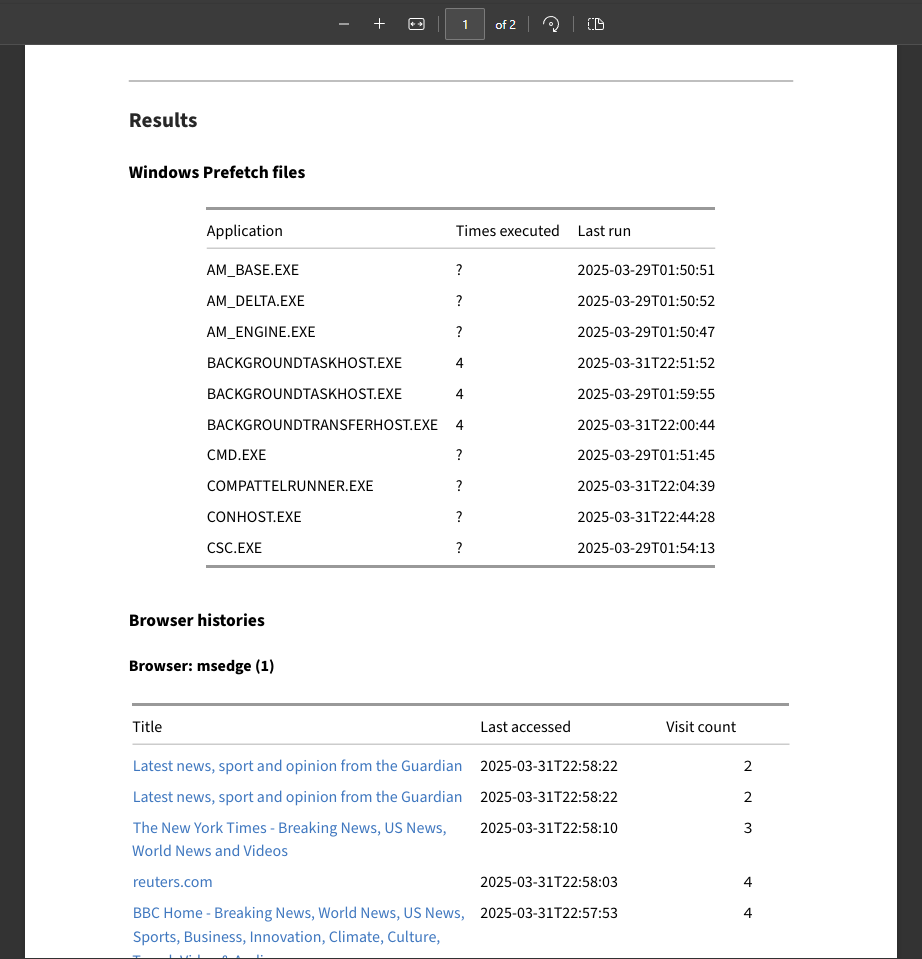
\includegraphics[width=1\linewidth]{human-reporting.png}
\caption{Sample PDF report generated by AKF
renderers}\label{fig:scenario-report}
\end{figure}

Of course, other options exist for generating human-readable (and
machine-readable) reporting from an AKF-generated dataset. For example,
the analysis features provided by tools such as Plaso
\cite{Log2timelinePlaso2025} and those developed by Eric Zimmerman
\cite{zimmermanEricZimmermansTools} can be used to supplement the
existing reporting and validation features of AKF. These tools can be
directly integrated into AKF workflows in the future, although this is
not currently the case.

After generating the scenario itself and any metadata and reporting that
should be included with the dataset, the challenge of distributing this
information remains. More precisely, how do we make our dataset as
accessible, reusable, and discoverable as possible?

\section{Distribution and community
reproducibility}\label{distribution-and-community-reproducibility}

A key challenge identified by Grajeda et al.~was the difficulty in
reproducing results in the field of digital forensics. While this is
primarily attributed to the \emph{availability} of forensic datasets in
general, it can also be attributed to challenges in the
\emph{reproducibility} of creating synthetic datasets.

Before addressing the low-level use of AKF as part of \autoref{chapter-six}, we will briefly discuss the infrastructure needed
to support community usage of the outputs of AKF scenarios and synthetic
datasets as a whole. Note that for the remainder of this section,
scenarios and datasets are both implied to be synthetic, as the
principles of reproducibility are less applicable to real-world
datasets.

There are four elements that must be distributed with a scenario to make
a dataset (and its results) reproducible:

\begin{itemize}
\tightlist
\item
  Any core outputs or individual artifacts generated from the virtual
  machine.
\item
  Any metadata, ground truth, or other reporting that describes the
  scenario.
\item
  The OS-specific ``base image'' used to create the dataset, typically a
  virtual machine with a newly installed operating system on which all
  synthesizer actions are performed.
\item
  The precise instructions required to build the scenario from the
  provided base image, whether human- or machine-readable instructions.
\end{itemize}

Forensic datasets have long included core outputs and individual
artifacts well before the development of AKF and other synthesizers;
there is limited value in a forensic scenario without anything to
analyze. Various forms of ground truth have also long been a part of
forensic datasets in multiple forms; some educational datasets include
PDF answer keys, while some research datasets have been labeled in a
structured format to include metadata about the dataset.

However, less common are detailed instructions to build the overall
scenario. Manually constructed datasets rarely describe the actions
taken to create a scenario in detail; for example, the educational
M57-Patents scenario built by Woods et al.
\cite{woodsCreatingRealisticCorpora2011} provides an instructor PDF
with a high-level timeline of actions taken in English. This detail is
sufficient for educational purposes but is too imprecise to guarantee
that others following this timeline will construct the disk image in the
same manner as intended. As described in \autoref{challenges-in-developing-synthetic-datasets},
non-determinism can be acceptable and even desirable in educational
contexts but is less desirable for tool validation and research.

Even rarer in manually constructed datasets is the inclusion of a base
image representing the machine's state before any actions are performed.
This may be attributable to both copyright concerns and a perception
that knowledge of the operating system alone is sufficient to rebuild
the base image; while it is true that setting up a virtual machine is
straightforward, any need for human interpretation introduces a source
of non-determinism that could be eliminated.

Synthesizers significantly improve on the lack of precise instructions;
their machine-readable scripts both document and execute the exact
instructions needed to reconstruct a scenario. However, this depends on
the availability of an OS- and synthesizer-specific base image; many
synthesizers expect their users to follow a set of human-readable
instructions to prepare a virtual machine specifically for use with that
synthesizer.

Where copyright issues are not a concern, synthetic images should aim to
include a complete definition of a virtual machine to be used as the
base image. A base image may be a full, hypervisor-specific virtual
machine (archiving and compressing the entirety of the associated
virtual machine folder), a hypervisor-independent virtual appliance (in
a format such as OVF), or another infrastructure-as-code solution to
define and build virtual machines, such as Vagrant.

AKF is designed to provide all four of these elements in every scenario
it creates; elements 1, 2, and 4 are inherent to AKF's design, while
base images can be provided as Vagrantfiles as described in \autoref{setup-and-basic-usage}. This ensures the
reproducibility of both the creation of AKF datasets and any results
derived from them.

Although not explored as part of this thesis, the inclusion of all four
of these elements as part of a well-structured, standardized
distribution format could be used to build a distribution platform
similar to CFReDS but with more powerful discovery and querying
functionality. While the contents of the scenario are primarily
described by CASE, it may also be possible to perform queries based on
the contents of Vagrantfiles and AKF scripts. For example, a user may
want to search for all images that use the agent-based Chromium artifact
generation described in \autoref{akf-implementation}, which can be achieved by searching for the inclusion of
the relevant AKF libraries in the scenario's scripts. However, this does
not address the challenge of storing and distributing scenarios
efficiently to support such a platform; this is discussed in
\autoref{distribution}.

With the reproducibility and value of AKF-generated scenarios
established, we now discuss how to invoke and leverage the underlying
technologies that provide these benefits.
